\section{Evaluation}\label{C:eval}

\subsection{Validity of refactorings}\label{S:validity}

We wrote 85 tests to ensure that the refactoring tool~\cite{rrproject} functions as expected. We test that either refactoring aborts or gives the expected output.

\subsubsection{Validity of renamings}

The test suite tests both the cases where a renaming should occur, and cases where it should not due to the variations in conflict types as outlined in Section~\ref{C:back}. Currently there are around 60 tests specifically written to test renaming, spread across the different classes of renaming. In particular, tests try to cause conflicts between the different classes, e.g., variable names with type names. We can examine a generic rename in Figure \ref{Fig:walk}. When running any of the renaming refactorings, name resolution will run to find any super-block conflict. Afterwards, any sub-block conflicts will be caught in a compilation run. 

\begin{figure*}
{\verb|let a = 2; // 1. Super-block conflict: caught by name resolution|}

{\verb|    {|}

{\verb|        let |}{\color{red}\verb|a|}{\verb| = 3;|}

{\verb|        let a = 4;|}

{\verb|        let b = |}{\color{red}\verb|a|}{\verb|; // 2. Sub-block conflict: caught by a compilation run|}

{\verb|    }|}
\caption{Examining a tentative rename in red}
\label{Fig:walk}
\end{figure*}

\paragraph{Methods and functions}
There are several tests for renaming methods defined with a trait and/or overridden by an implementing struct. Tests address both static and dynamic dispatch. One known failure mode of the refactoring tool is when a function (or trait) is declared within a function scope.

\paragraph{Concrete types -- structs and enums}
There are tests for both renaming of structs and enums with detection of namespace collisions (which are not in local scopes). The checking of namespace collisions also extend to the usage of `use' imports which allow a specific namespace to be imported and no need to additionally qualify some names. The renaming of concrete types does not extend to type aliases, although the extent of partial support is unknown.

\paragraph{Examining a particular edge case}
Figure \ref{Fig:fix} shows an edge case identified during this project. A struct {\verb|Point|} with fields {\verb|x|} and {\verb|y|} can be used to initialize two corresponding local variables {\verb|x|} and {\verb|y|}. Without intervention, a local variable renaming might attempt to change {\verb|x|} to  {\verb|foo|} but {\verb|Point|} has no corresponding field {\verb|foo|}. 

\begin{figure}
\begin{verbatim}
// Before refactoring
let Point{x, y} = Point{x:1, y:2}
// After refactoring (invalid):
let Point{foo, y} = Point{x:1, y:2}
// Manually user-corrected (valid)
let Point{x:foo, y:y} = Point{x:1, y:2}
\end{verbatim}
\caption{Invalid rename of \emph{x} to \emph{foo} which is easily fixed manually}
\label{Fig:fix}
\end{figure}

\subsubsection{Examining inline-local}
The inline-local refactoring is at proof-of-concept stage. The majority of the work on this refactoring has been in exploring and describing the knowledge gained. While there is some obvious checking, without an `effect' system and pure functions, there is a good deal of missing validation. Arguably, the situation is not much better than any other languages that don't bother with mutability or ownership at all.

\subsubsection{Examining elide-reify}

We are confident (supported by tests) that the lifetime reification refactoring is correct and complete.

Lifetime elision is mostly correct but incomplete. It fails in compex cases, such as when only some lifetimes may be elided or lifetimes used as bounds on traits. Since this is a new refactoring, exactly how useful the reification and elisions are, is unknown.

\subsubsection{Formal correctness and alternative approaches}

Formal foundations for refactoring in general appears incredibly weak as raised by the JRRT~\cite{schafer2010specification} paper. Even the most trivial of refactorings often lack written specification and are based solely on implementation. One related case study includes a graph rewriting approach to refactoring simple programs~\cite{graph} which achieves reasonable success, but they note in their discussion the difficulties of handling language specific features (highlighting a massive limitation). Another recent paper from the Haskell community reiterates the difficulty of implementing a concrete refactoring tool or even understanding what should and should not be considered a ``valid refactoring''~\cite{sculthorpe}. It appears that, the act of implementing a reasonably powerful refactoring tool is no easy feat on its own leave alone stating its specifications or formal properties it might guarantee.

\subsection{Performance evaluation}\label{S:perfeval}
With only single file tests, the amount of time spent performing each refactoring is negligible. Compilation times for single files, particularly trivial programs do not provide sufficient evidence of practical timing for performing a refactoring. Therefore we investigated real world code from  crates.io, the Rust package repository \cite{cratesio15}. 

\subsubsection{Relative crate sizes}
Figure \ref{Fig:codesize} lists  four crates from crates.io that have been chosen to help evaluate our tool. The crates are four of the five most downloaded crates by the Rust community \cite{cratesio15}. The `winapi' crate was omitted due to less relevance on a Linux platform. The lines of code metric counts only Rust source (.rs) files, but does not discount comments or test code. The purpose of the comparison is only to generate a rough idea of the size of the crates.

\begin{figure}[h]
\begin{center}
    \begin{tabular}{ | l | c |}
    \hline
    \textbf{Rust crate} & \textbf{Lines of code} \\ \hline
    libc & 6547 \\ \hline
    rustc-serialize &  5741 \\ \hline
    rand &   5187 \\ \hline
    log &  1449 \\ \hline
    \end{tabular}
\end{center}

\caption{Size of crates compared}
\label{Fig:codesize}
\end{figure}

\subsubsection{Comparing the timings between the types of refactorings}
Timings were generated for the different crates using the Linux perf tool: {\verb|perf stat -r 10|} Timings were averaged over 10 runs and use of the perf tool gave much smaller unaccountable variations in results compared to other tools such as {\verb|time|}. The machine used was a dual core 2.0 GHz machine running Ubuntu 12.04 with Rust Nightly 23/09/2015. The tool was compiled in release (i.e., optimised) mode which ensures increased speed, around 10x based on observation (relative to debug, un-optimised, mode). Timings represent elapsed time, not system time or CPU time.

The classes of refactorings measured are: renaming variables, renaming functions, renaming types, lifetime reification and lifetime elision. Inline local has been omitted due to lack of sufficient examples in the given crates, particularly without mutation. In each case, examples were picked with effectively a single usage, access or equivalent (with minimal modifications made) so that the difference in timings between each of the individual refactorings could be highlighted. Figure \ref{Fig:compareref} shows how, regardless of refactoring, the time taken is generally comparable within a crate. Looking at Figure \ref{Fig:codesize}, the blind code size metric does not appear to be a good indicator of the base refactoring time and so comparisons between crates are limited. In general, the complexity of a crate is not necessarily tied to crate size. Function renaming takes noticeably longer, while lifetime refactorings are noticeably quicker. This bis linked to the basic compile time. While a rename refactoring requires checking every usage of a declared item using the compiler, in the `happy path' every usage should fail the compiler check during the early stages of name resolution. Only in more unlikely or unfortunate cases will a refactoring require any additional processing in analysis.

\begin{figure}[h]
\begin{center}

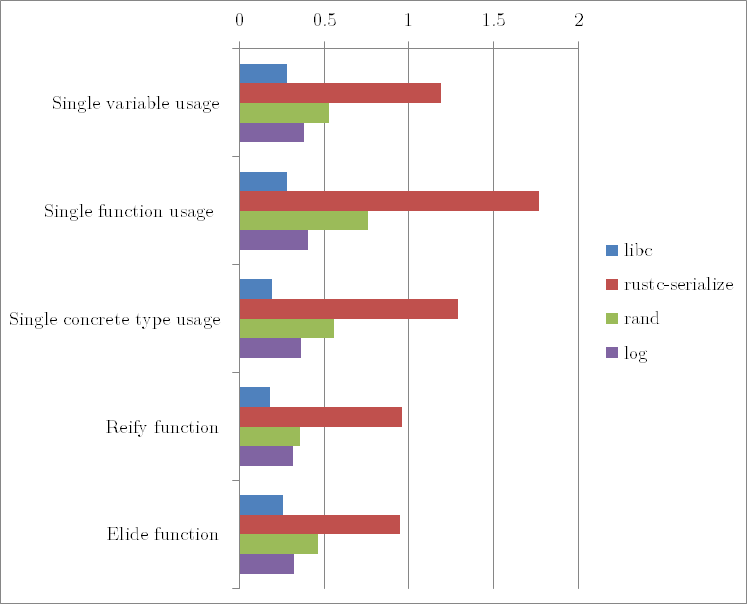
\includegraphics[width=8cm]{refactorings}

\caption{Graph displaying timing in seconds for the different refactorings}
\label{Fig:compareref}
\end{center}
\end{figure}

\subsubsection{Varying the number of refactoring locations or usages}
From `libc', a number of different concrete types were targeted for performing a rename. `libc' was chosen for having a wider variety of occurrence counts specifically with concrete types. Figure \ref{Fig:comparerefs} shows how concrete type renaming appears to scale linearly (as expected from Sect. \ref{C:impl}) with the number of usages. Ideally, this analysis would have been done with other refactorings, but finding a reasonable amount of variation on the number of usages was difficult and searching was mostly manual. All the rename refactorings generally follow similar code paths and so the idea is that they should all scale in the same way (with the same general relationship). In particular, investigating function renaming would have been insightful as they take inherently more time. Although we expect to always scale linearly with the number of usages, the entire compiler is invoked each time instead of running what is actually necessary, like name resolution. As such, improvements can likely be made to the multiplying factor. As for the lifetime refactorings, the selection for the earlier timings did not strongly consider the number of visible `\&' and from observation, the time they took did not generally vary significantly. This is probably because they do not use additional passes of the compiler. Investigating scalability allows us to predict the time required for refactoring larger codebases. Referring back to Fowler, this is important for a tool since taking too long means that a programmer would simply prefer to do the refactoring by hand.

\begin{figure}[h]
\begin{center}
    \begin{tabular}{ | l | c |}
    \hline
    \textbf{Number of replaced occurrences} & \textbf{Time in seconds} \\ \hline
    1 type usage &  0.1925  \\ \hline
    3 type usages &  0.3821  \\ \hline
    4 type usages &   0.4749  \\ \hline
    6 type usages &   0.6737  \\ \hline
    8 type usages &   0.8739 \\ \hline
    13 type usages  &  1.373 \\ \hline
    29 type usages &  2.960  \\ \hline
    51 type usages &  5.059 \\ \hline
    \end{tabular}
\end{center}

\caption{Timings for varying usage counts of concrete types in libc}
\label{Fig:scaling}
\end{figure}

\begin{figure}[h]
\begin{center}

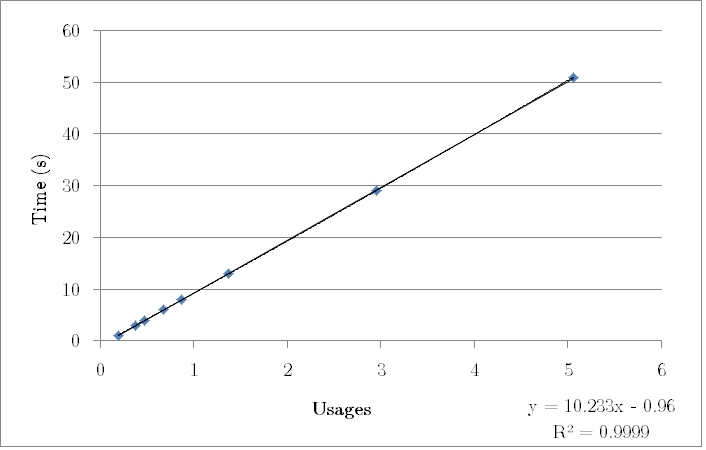
\includegraphics[width=8cm]{scaling}

\caption{Graph displaying results of varying the number of usages}
\label{Fig:comparerefs}
\end{center}
\end{figure}